\chapter{Performnce Evaluations}\label{chap:performance}

In this chapter we present an evaluation of the 
performance of our MLMC implementations for the Stochastic Heat Equation 
and Dean-Kawasaki equations outlined in the previous chapter. 
We aim to quantify the computational savings achieved by the MLMC 
method relative to the standard Monte Carlo estimator, 
and to compare the relative performance savings of different
noise coupling strategies within the MLMC framework.
Before presenting results, we outline how present the performance
is measured.

Performance is measured using the dimensional metric 
$$
\mathrm{Cost} \times \varepsilon^2,
$$ 

where $\varepsilon$ is a target RMSE and Cost is taken to be the measured wall-clock runtime.
This is similar to the performance measurement approach used in 
These results were gathered using code written in C++ 
and used the standard C++11 Mersenne 
Twister PRNG \cite{cpp20standard}. All experiments were executed 
on Intel Gold 6538Y+ processors \cite{intel_xeon_gold_6538y}.

\begin{figure}[htbp]
    \centering
    \begin{subfigure}{0.45\textwidth}
        \centering
        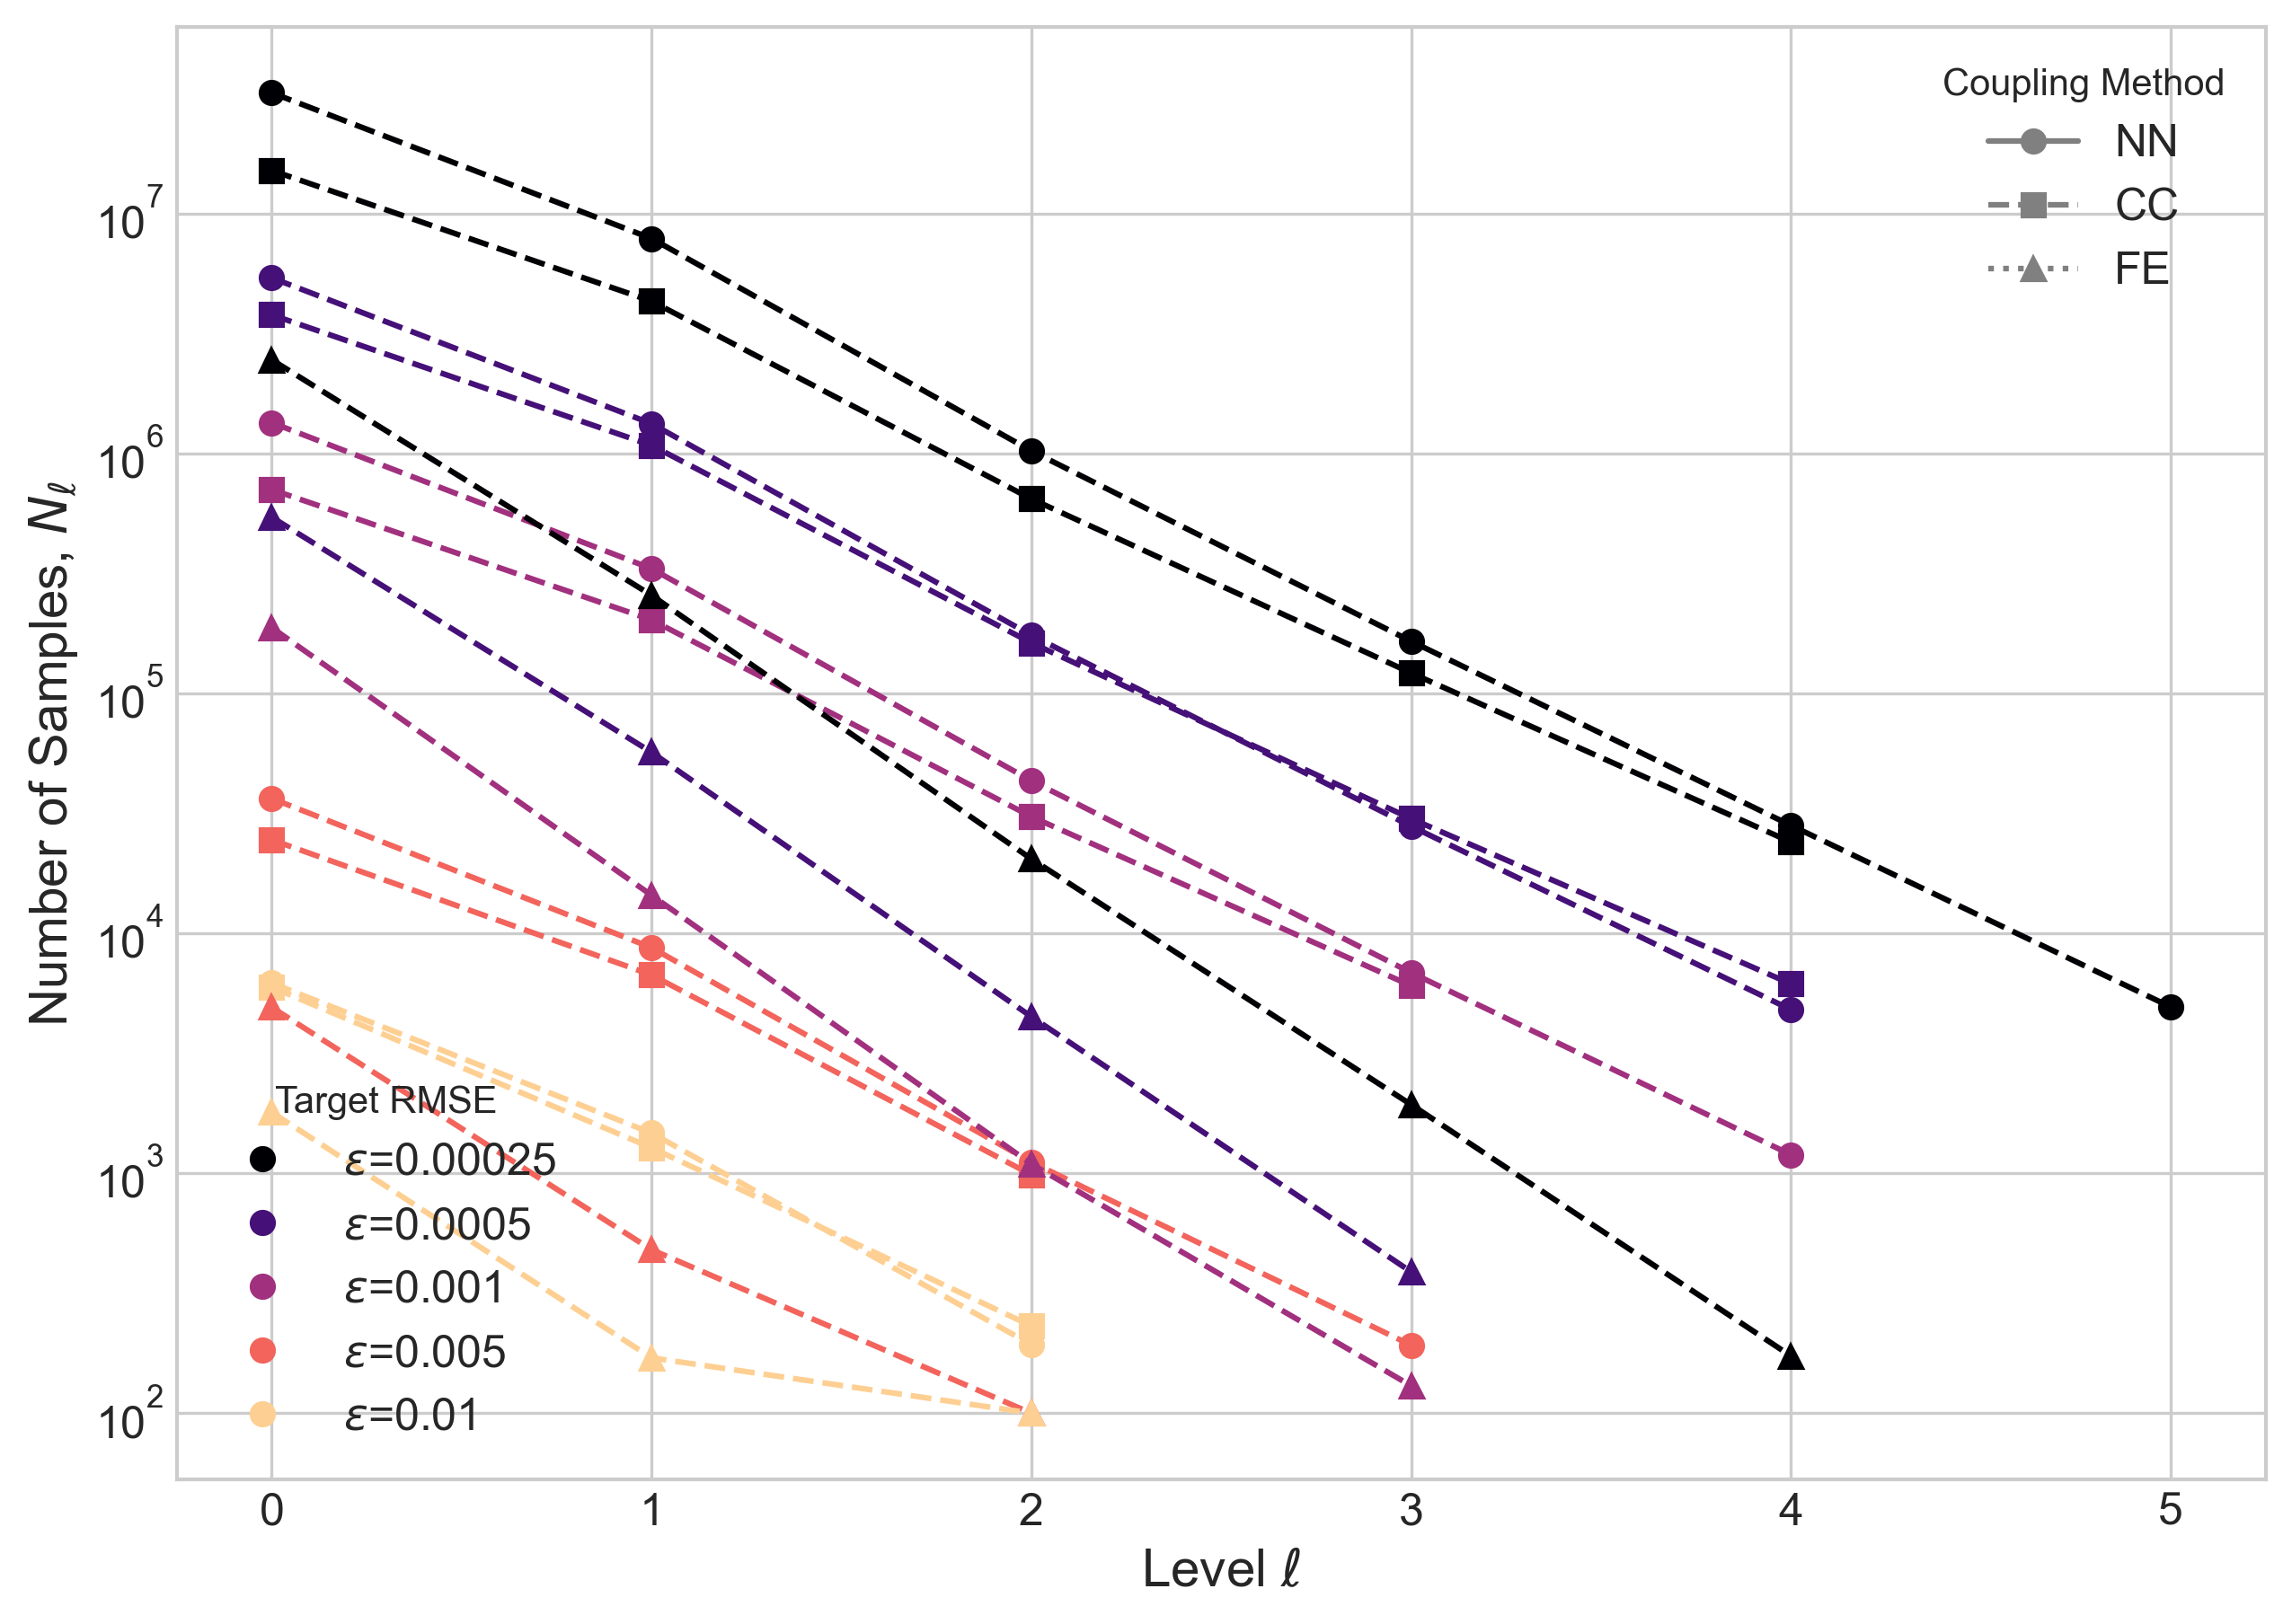
\includegraphics[width=\linewidth]{graphics/she_sq_amps_nums.png}
        \caption{First plot}
        \label{fig:plot1}
    \end{subfigure}
    \hfill
    \begin{subfigure}{0.45\textwidth}
        \centering
        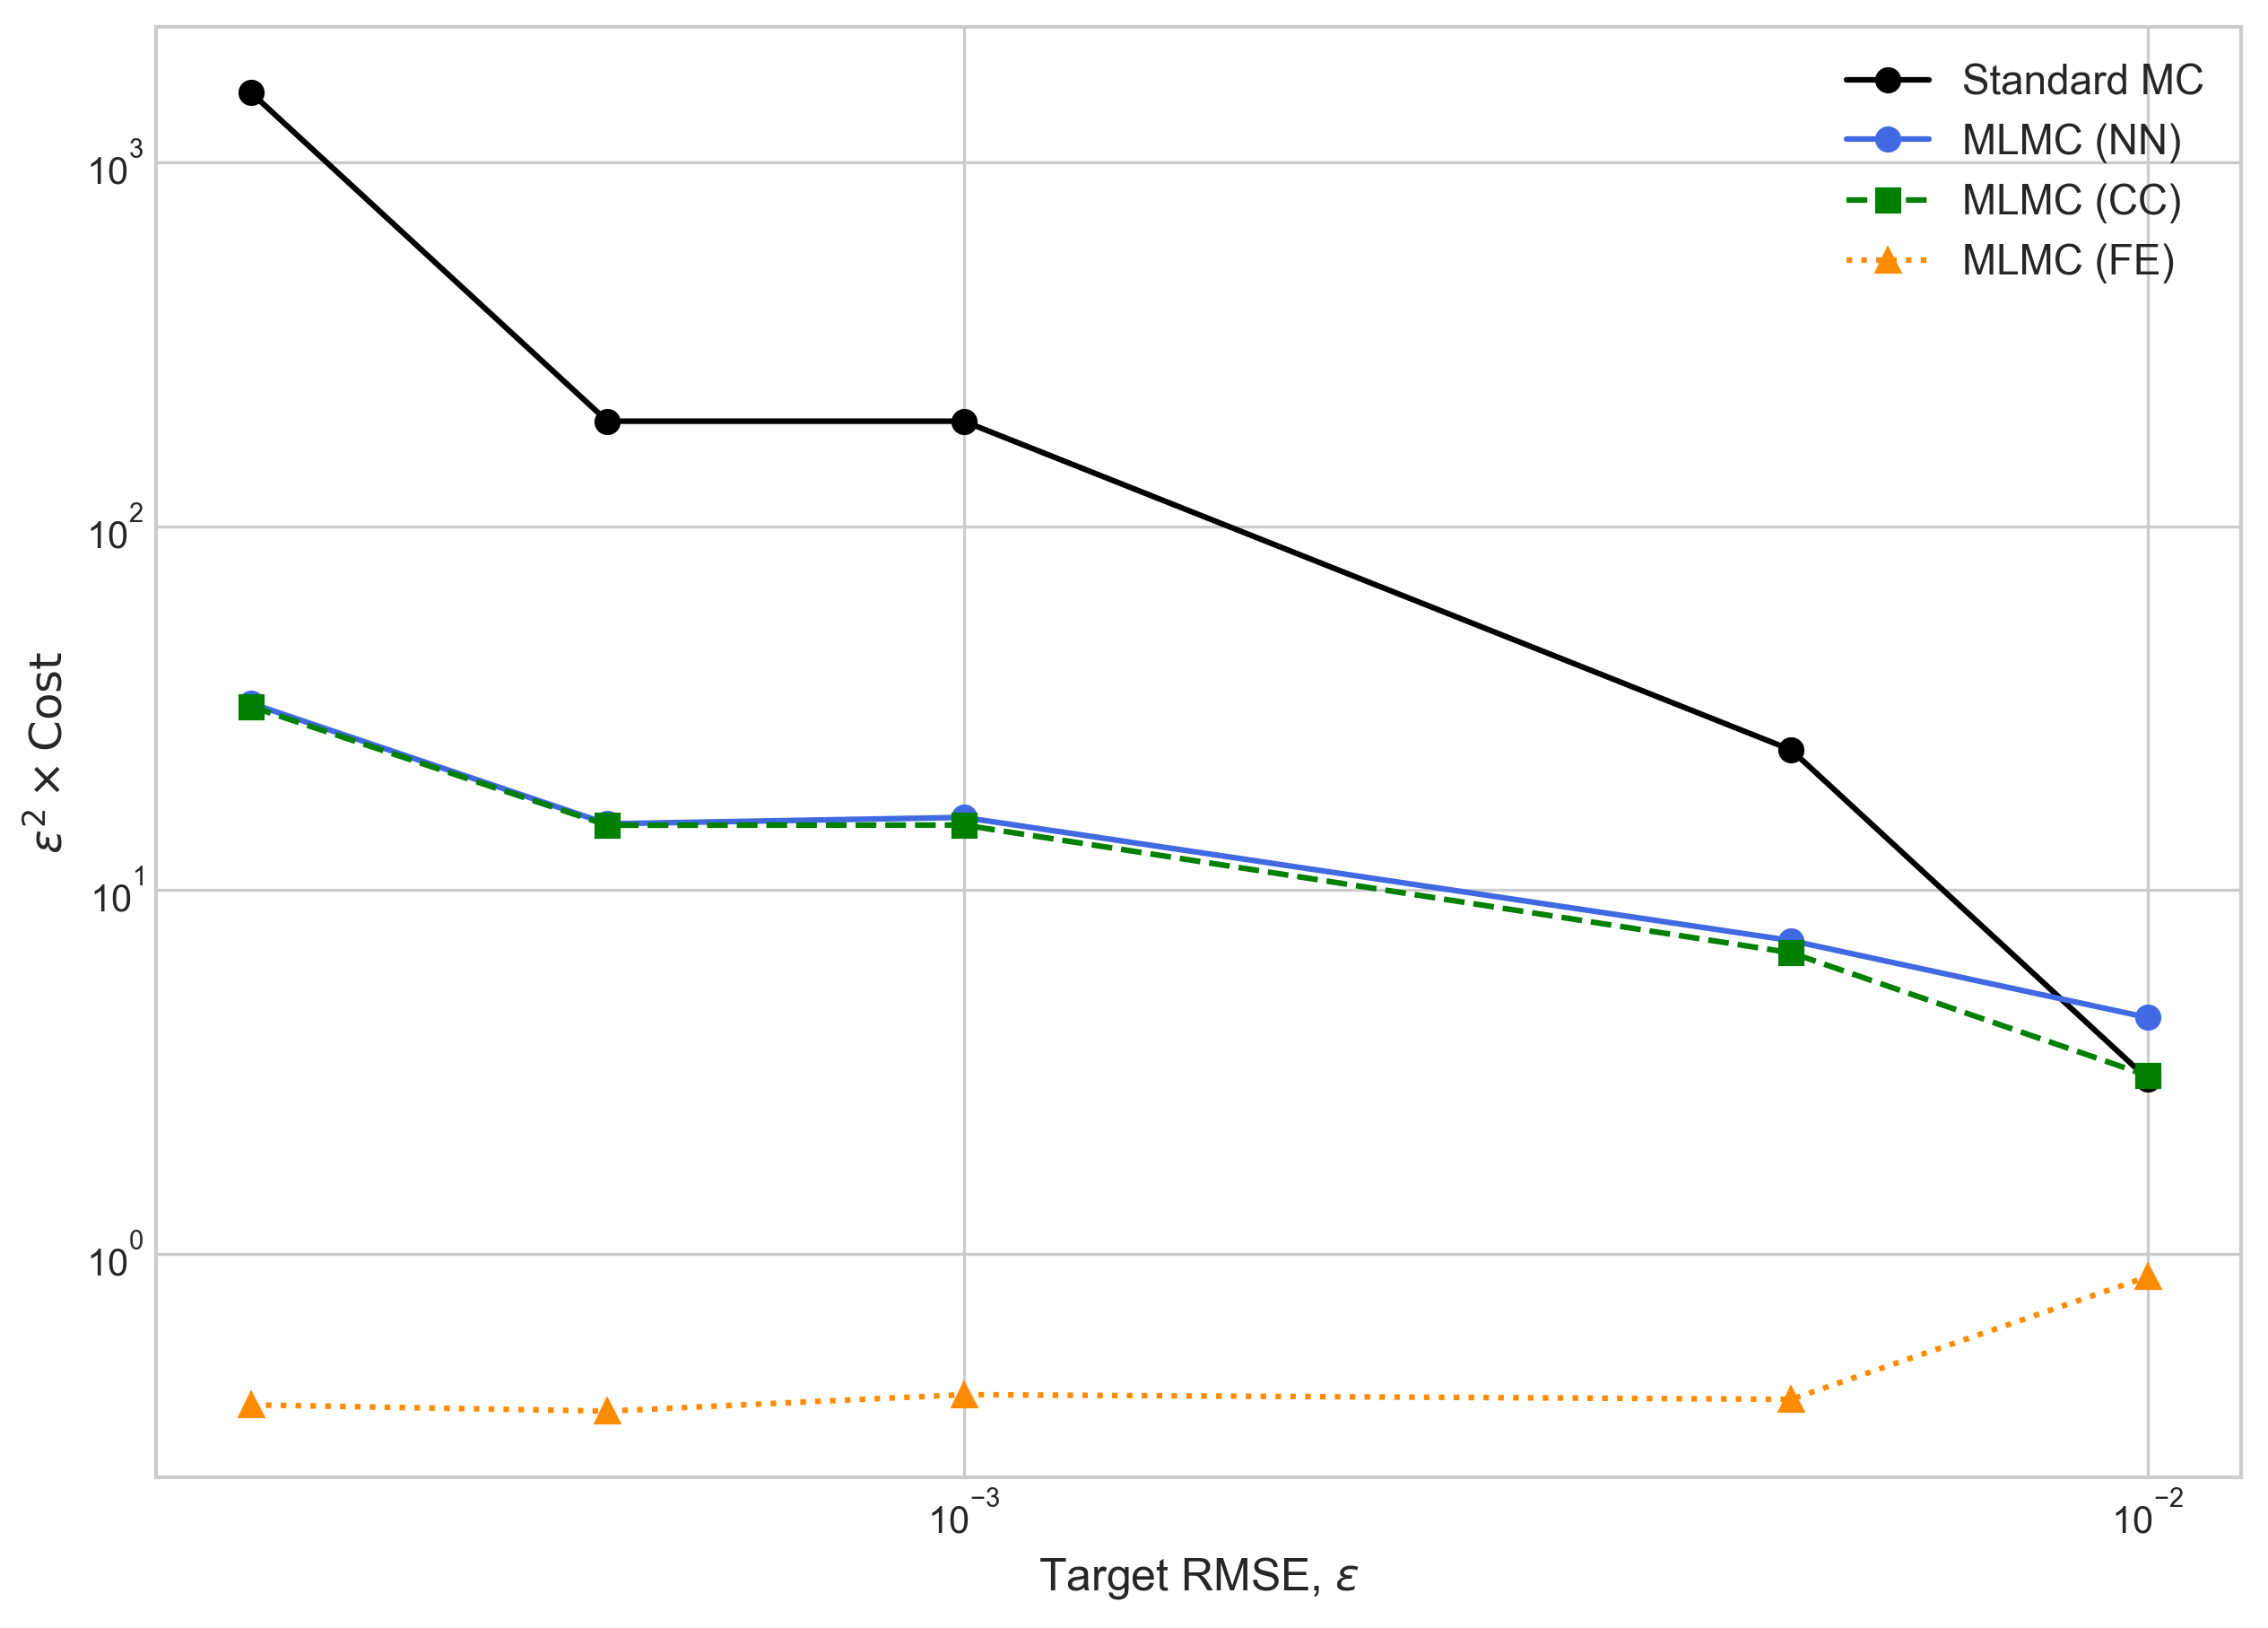
\includegraphics[width=\linewidth]{graphics/she_sq_amp_costs.png}
        \caption{Second plot}
        \label{fig:plot2}
    \end{subfigure}
    
    \begin{subfigure}{0.45\textwidth}
        \centering
        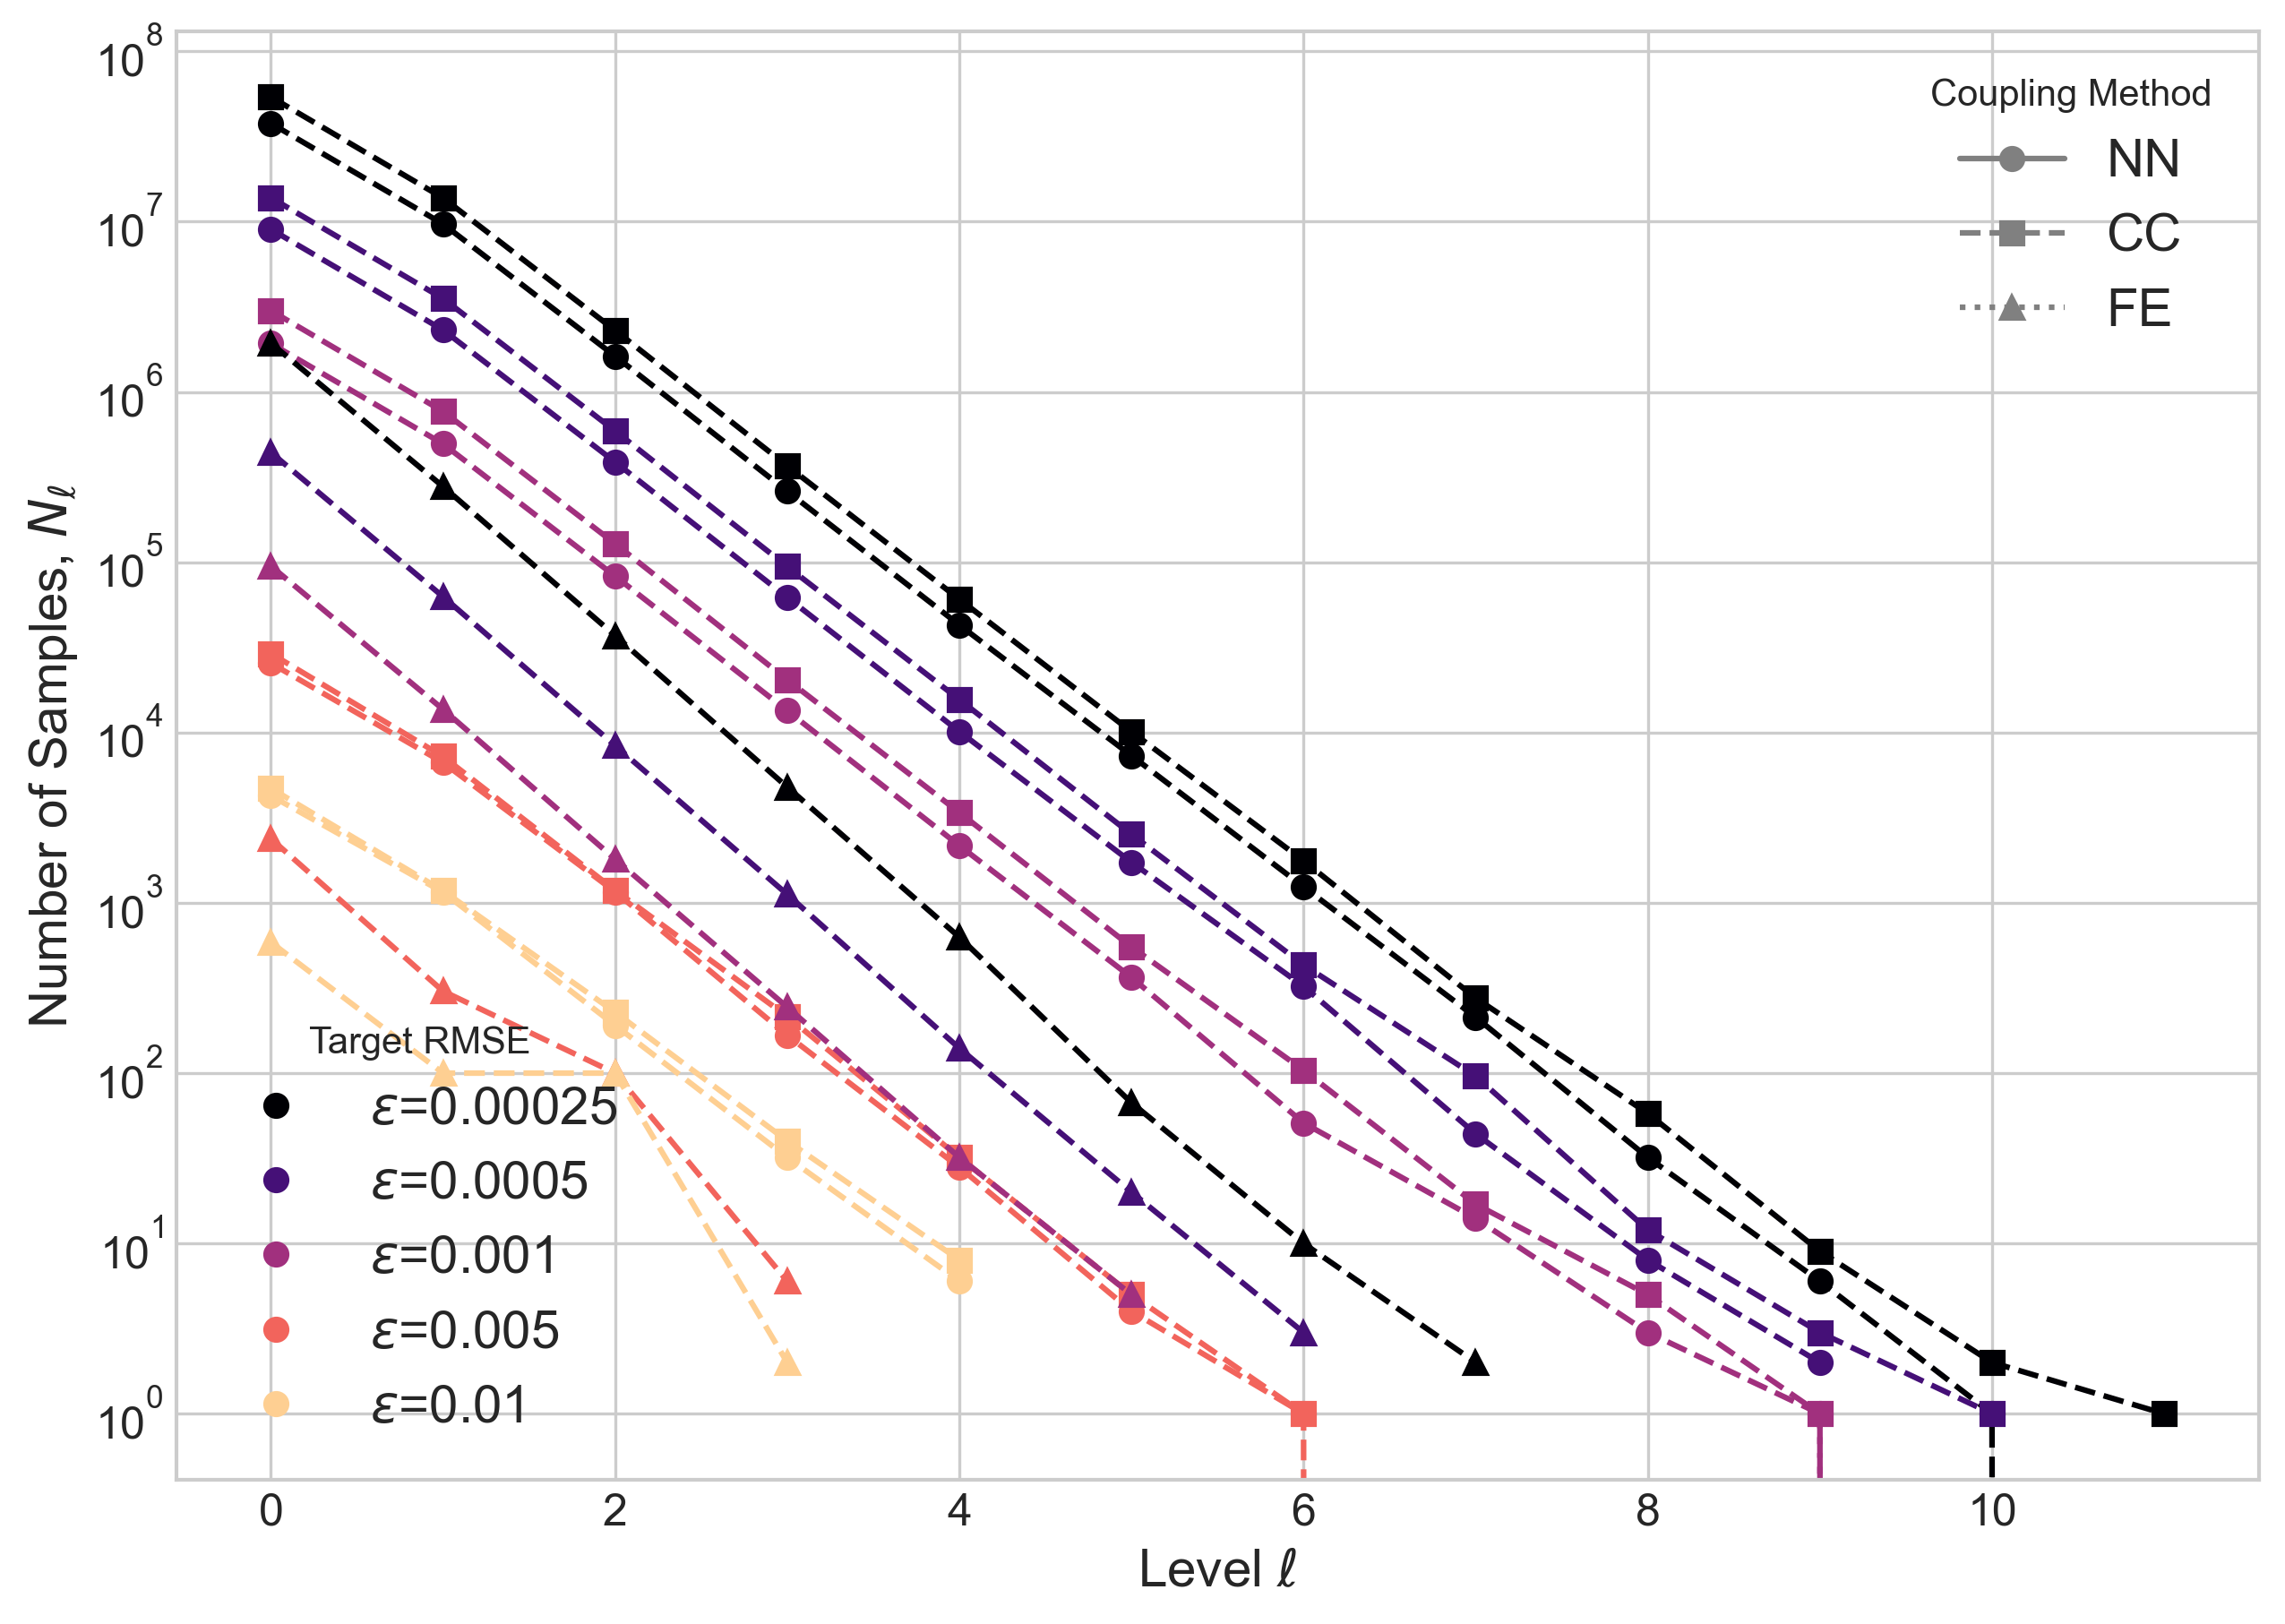
\includegraphics[width=\linewidth]{graphics/she_energy_nums.png}
        \caption{Third plot}
        \label{fig:plot3}
    \end{subfigure}
    \hfill
    \begin{subfigure}{0.45\textwidth}
        \centering
        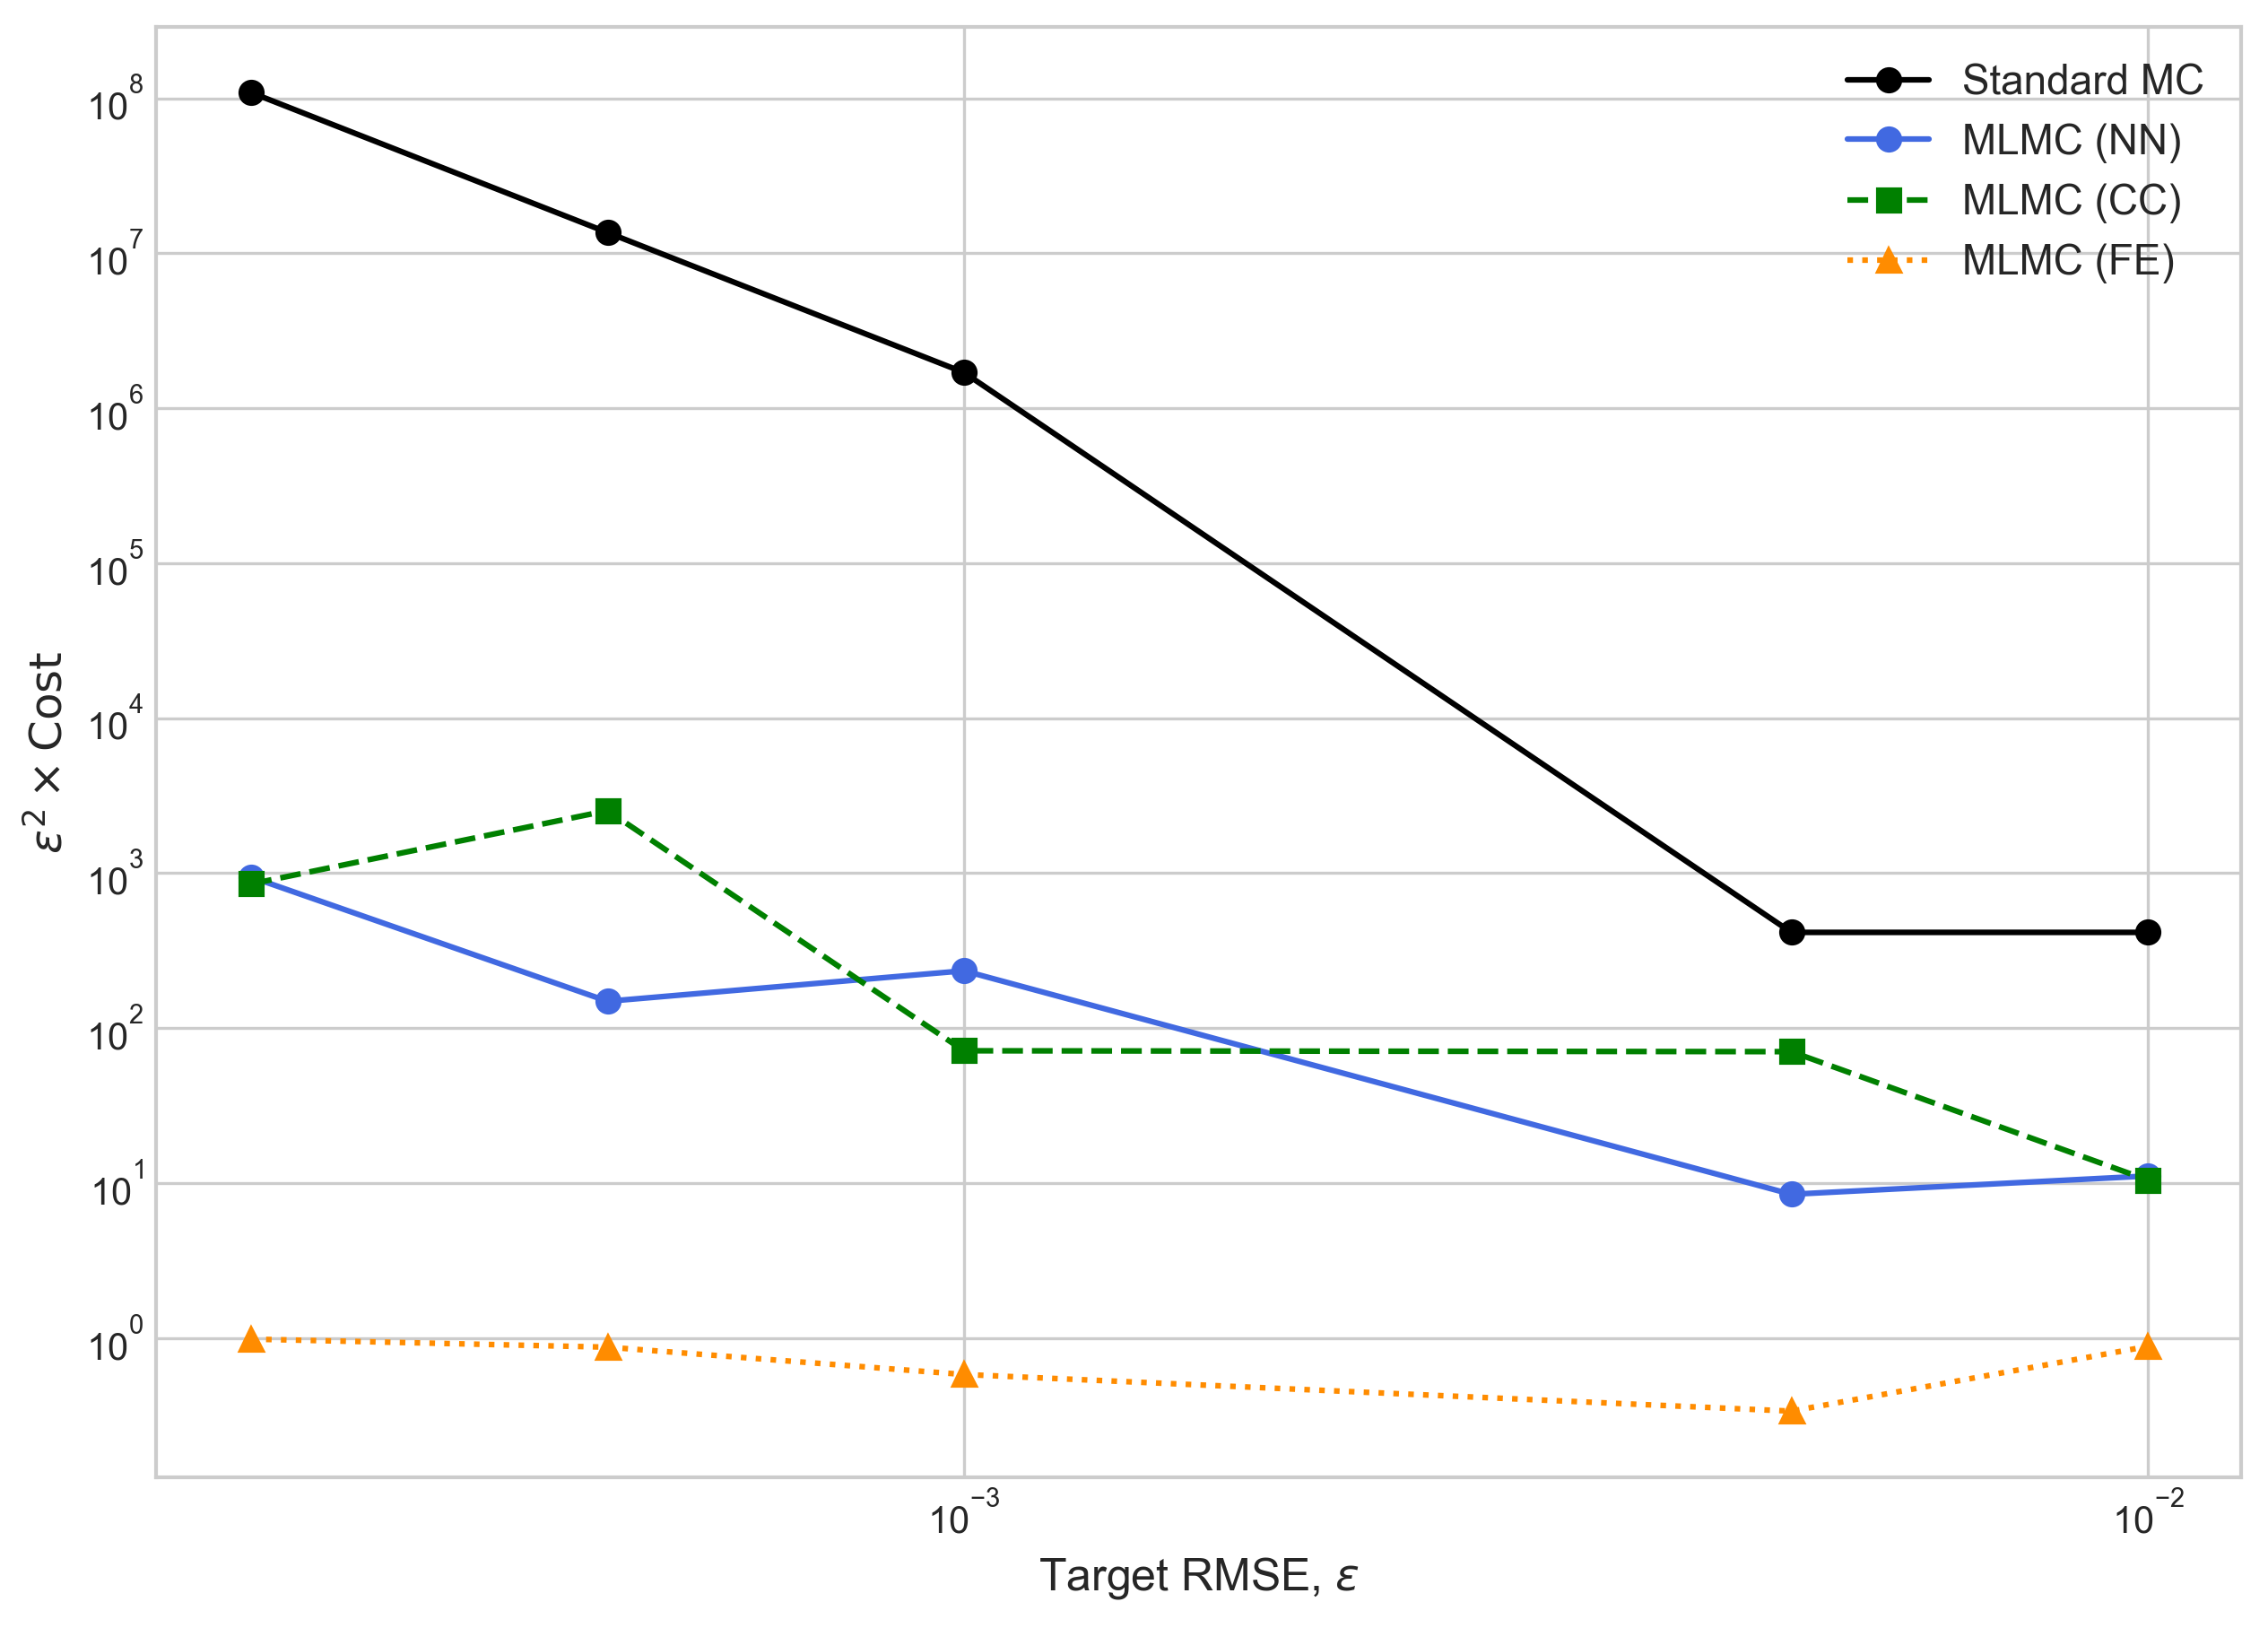
\includegraphics[width=\linewidth]{graphics/she_costs.png}
        \caption{Fourth plot}
        \label{fig:plot4}
    \end{subfigure}

    \caption{A 2 by 2 grid of plots.}
    \label{fig:2by2plots}
\end{figure}
